%%%%%%%%%%%%%%%%%%%%%%%%%%  ltexpprt.tex  %%%%%%%%%%%%%%%%%%%%%%%%%%%%%%%%
%
% This is ltexpprt.tex, an example file for use with the SIAM LaTeX2E
% Preprint Series macros. It is designed to provide double-column output.
% Please take the time to read the following comments, as they document
% how to use these macros. This file can be composed and printed out for
% use as sample output.

% Any comments or questions regarding these macros should be directed to:
%
%                 Donna Witzleben
%                 SIAM
%                 3600 University City Science Center
%                 Philadelphia, PA 19104-2688
%                 USA
%                 Telephone: (215) 382-9800
%                 Fax: (215) 386-7999
%                 e-mail: witzleben@siam.org


% This file is to be used as an example for style only. It should not be read
% for content.

%%%%%%%%%%%%%%% PLEASE NOTE THE FOLLOWING STYLE RESTRICTIONS %%%%%%%%%%%%%%%

%%  1. There are no new tags.  Existing LaTeX tags have been formatted to match
%%     the Preprint series style.
%%
%%  2. You must use \cite in the text to mark your reference citations and
%%     \bibitem in the listing of references at the end of your chapter. See
%%     the examples in the following file. If you are using BibTeX, please
%%     supply the bst file with the manuscript file.
%%
%%  3. This macro is set up for two levels of headings (\section and
%%     \subsection). The macro will automatically number the headings for you.
%%
%%  5. No running heads are to be used for this volume.
%%
%%  6. Theorems, Lemmas, Definitions, etc. are to be double numbered,
%%     indicating the section and the occurence of that element
%%     within that section. (For example, the first theorem in the second
%%     section would be numbered 2.1. The macro will
%%     automatically do the numbering for you.
%%
%%  7. Figures, equations, and tables must be single-numbered.
%%     Use existing LaTeX tags for these elements.
%%     Numbering will be done automatically.
%%
%%  8. Page numbering is no longer included in this macro.
%%     Pagination will be set by the program committee.
%%
%%
%%%%%%%%%%%%%%%%%%%%%%%%%%%%%%%%%%%%%%%%%%%%%%%%%%%%%%%%%%%%%%%%%%%%%%%%%%%%%%%



\documentclass[twoside,leqno,twocolumn]{article}
\usepackage{ltexpprt}

%jing
\usepackage{graphicx}
\usepackage{balance}  % for  \balance command ON LAST PAGE  (only there!)
%
\usepackage{amsmath,amssymb}
%\usepackage[ruled]{algorithm2e}
\usepackage{xcolor}
\usepackage{caption2}
%\usepackage{verbatim}
\usepackage{url}
%%wj\usepackage{paralist}
%%wj\usepackage{lstautogobble}
%%wj\usepackage{listings}
%
%\usepackage{subcaption}
\usepackage{amsmath}
%\usepackage{bbold}
\usepackage{subfigure}
%\usepackage{enumitem}
\usepackage{textcomp}
%\usepackage{graphicx}
\usepackage{multirow}
\usepackage{comment}
\usepackage{algorithm}
\usepackage{algpseudocode}
\usepackage{booktabs}

\begin{document}


%jing
\newtheorem{definition}{Definition}
\newtheorem{problem}{Problem}
%\newtheorem{theorem}{Theorem}
\newtheorem{remark}{Remark}
%\newtheorem{lemma}[theorem]{Lemma}
%\newtheorem{corollary}[theorem]{Corollary}
%
\newcommand{\sys}{\textcolor{blue}{\uppercase{G}\lowercase{ru}\uppercase{B}\lowercase{a}}}
\newcommand{\tbc}{\textcolor{blue}{[To Be Completed]}}
\newcommand{\refe}{\textcolor{blue}{[reference]}}
\newcommand{\retg}{\textcolor{blue}{retweeting}}
\newcommand{\retgs}{\textcolor{blue}{retweetings}}
\newcommand{\Retg}{\textcolor{blue}{Retweeting}}
\newcommand{\retd}{\textcolor{blue}{retweeted}}
\newcommand{\ret}{\textcolor{blue}{retweet}}
\newcommand{\od}{\textcolor{blue}{O's Distance}}
\newcommand{\hd}{\textcolor{blue}{H's Distance}}
\newcommand{\gd}{\textcolor{blue}{G's Distance}}
%%jing


%\setcounter{chapter}{2} % If you are doing your chapter as chapter one,
%\setcounter{section}{3} % comment these two lines out.


\title{\Large Incorporating User Grouping into \Retg{} Behavior Modeling\thanks{Supported by NSFC (U1636210), 973 program(2014CB340300), NSFC (61322207\&61421003), Special Funds of Beijing Municipal Science \& Technology Commission, Beijing Advanced Innovation Center for Big Data and Brain Computing, and MSRA Collaborative Research Program.}}
\author{Author 1\thanks{affiliation} \\
\and
Author 2\thanks{affiliation}}
\date{}	


\maketitle

% Copyright Statement
% When submitting your final paper to a SIAM proceedings, it is requested that you include 
% the appropriate copyright in the footer of the paper.  The copyright added should be 
% consistent with the copyright selected on the copyright form submitted with the paper.
% Please note that "20XX" should be changed to the year of the meeting.

% Default Copyright Statement
\fancyfoot[R]{\footnotesize{\textbf{Copyright \textcopyright\ 2018 by SIAM\\
Unauthorized reproduction of this article is prohibited}}}

% Depending on which copyright you agree to when you sign the copyright form, the copyright 
% can be changed to one of the following after commenting out the default copyright statement
% above.

%\fancyfoot[R]{\footnotesize{\textbf{Copyright \textcopyright\ 20XX\\
%Copyright for this paper is retained by authors}}}

%\fancyfoot[R]{\footnotesize{\textbf{Copyright \textcopyright\ 20XX\\
%Copyright retained by principal author's organization}}}


%\pagenumbering{arabic}
%\setcounter{page}{1}%Leave this line commented out.

\begin{abstract}
%Social media applications are emerging, with rapidly growing users and large numbers of \retd{} microblogs every minute.
The variety among massive users makes it difficult to model their \retg{} activities.
Obviously, it is not suitable to cover the overall users by a single model. % \cite{IEEEexample:journals/tkdd/ZhangTLLX15,IEEEexample:conf/wsdm/FengW13,IEEEexample:conf/ijcai/ZhangLTCL13}.
Meanwhile, building one model per user is not practical.
To this end, this paper presents a novel solution, of which the principle is to model the \retg{} behavior over user groups.
Our system, \sys{}, consists of three key components for extracting user based features, clustering users into groups, and modeling upon each group.
Particularly, we look into the user interest from different perspectives including long-term/short-term interests and explicit/implicit interests.
%, which results deep analyses towards the \retg{} behavior and proper models in the end.
We have evaluated the performance of \sys{} using datasets of real-world social networking applications, showcasing its benefits.

\keywords{user grouping \middot social networks \middot behavior modeling}
\end{abstract}
% behavior and activity in this paper are interchangeable

\section{Introduction}
\label{sec:intro}

Social media is overwhelming nowadays, with massive users on Facebook \refe{}, Twitter \refe{} and Weibo \refe{} while the number of users keeps increasing.
These users behave variously, knowledge of which is significant in recommendation system, activity prediction and Big Thing analysis.
Hence emerges the demand of developing systems and algorithms that could properly model user behaviors, which has attracted the attention from both academia and industry.

Central to user behavior modeling, is the need to choose the unit of model (i.e., how many users share one model), as well as the variety of features to be selected for differentiating these units.
Already, there exist work of building a single model for all the users \refe{}.
Apparently, such model bears the limitation of being coarse.
On the other hand, modeling each user is not practical, due to the tremendous number of users.

The key driver of our work is the realization that in social media applications, users could fall into groups and each group shares representative behaviors.
Particularly, we study the \retg{} behavior of users and our work can be generalized to other behaviors of like and comment as well. 
As one example, consider the film \textit{Brave Heart}, fans of which are probably addicted to highland, bagpipe and war films, and thus likely to \ret{} blogs of these topics.

The contributions of this work include:
\begin{itemize}
\item We present a system named \sys{} with the novel perspective to model user behaviors over groups instead of the mono model in literature.
\item We leverage user interests to facilitate the modeling of \retg{} behavior and look into interests with various dimensions, including long-term/recent interests and explicit/implicit interests.
\item We evaluate the performance of \sys{} using real-world datasets, showcasing its benefits against competitive state of the art approaches.
\end{itemize}


The rest of this paper is organized as follows.
Section \ref{sec:overv} first gives the problem formulation and subsequently overviews \sys{}'s components, principle of which are detailed in Sections \ref{sec:fe}, \ref{sec:uc} and \ref{sec:gm} separately.
Section \ref{sec:perf} provides the performance evaluation.
Related work is presented in Section \ref{sec:rela}.
Finally, Section \ref{sec:conclu} concludes the work.












\section{Overview of System \sys{}}
\label{sec:overv}

\subsection{Problem Formulation}
% {user, blog, user-blog} => model
% query (a user u, a blog b that is created or forwarded by u's friend)
% returns: Y/N u shall forward b

\par We consider the \retg{} behavior of users in social media.
%For simplicity, with a given user, we assume that microblogs created or \retd{} by his/her followees cover the overall candidates, from which the said user may \ret{}.
For simplicity, assuming the microblogs that a user can \ret{} come from those owned by his/her followees.

%All our results could straightforwardly generalize to alternative candidate scopes.
%e.g., the like/unlike behavior against the candidate of remarking [double check the network language; register a Facebook]
%e.g., positive comments in the overall comments

\begin{definition}
\label{def:blog}
A microblog $M_b = (O, T, M, flag)$ has its owner $O$ (a.k.a. user in this paper) to whom $M_b$ belongs (either \twd{} or \retd{}), the generated time $T$ of $M_b$, the message context $M$, and $flag$ denoting $M_b$ is \retd{} or originally \tw{} by $O$. Here we use 1 and 0 to denote \retd{} and  \tw{}, respectively.
\end{definition}

\begin{comment}
\begin{definition}
A blog $B = (O, T, M, C)$ consists of the owner $O$ to whom $B$ belongs (either created or \retd{}), the timestamp $T$ showing when $B$ is generated, the blog message $M$ and a set of counters $C_s(B) = \{\#comment,\ \#like,\ \#\ret{}\}$ regarding the number of being commented, liked, and \retd{}.
\end{definition}
\end{comment}

\begin{definition}
\label{def:user}
Given a user $u$, we adopt $B_u$, $R_u$ and $E_u$ to represent her/his microblogs $B_u$, followers $R_u$ and followees $E_u$,  respectively, in which a follower/followee is a user.
\end{definition}

%The mapping between blog $B$ and user $U$ is a bilateral operation, i.e., $U = O(B)$ and $B \in B_s(U)$, through ID(s) of user and blog respectively.
Note that $M_b.O$ is a user, and $B_u$ is a set of microblogs.


Providing a set of users $\mathbb{U}$ and their associated microblogs $\mathbb{B}$, system \sys{} builds a \retg{} model for each group of  $\mathbb{U}$, such that given a microblog $b$ and a follower $f$ of its onwer $b.O$, i.e., $f \in R_{b.O}$, 1 or 0 is returned regarding whether $f$ \ret{s} $b$ or not.

\begin{figure}[tb!]
\centering
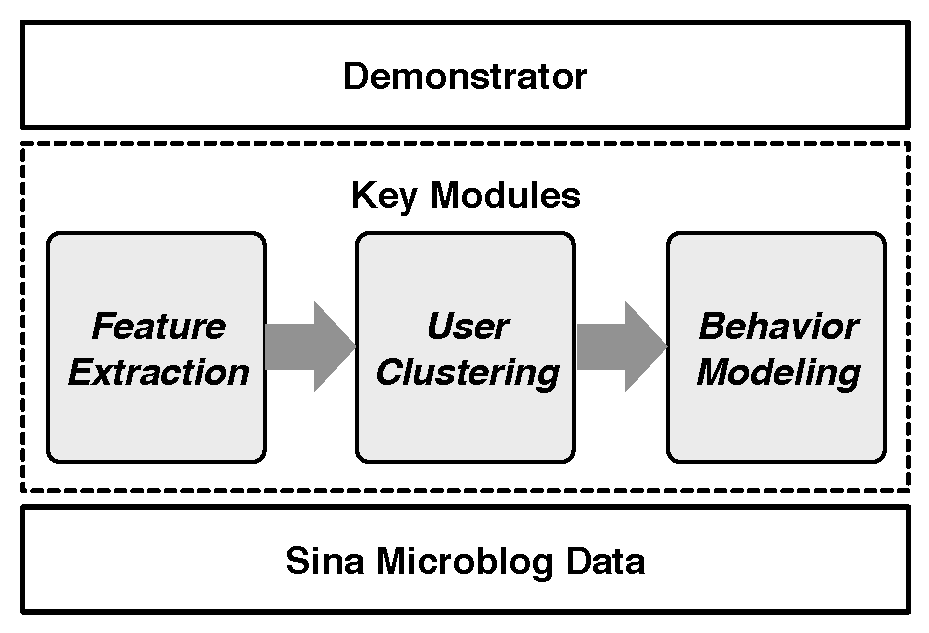
\includegraphics[width=.6\linewidth]{figures/architecture.eps}
%\vspace{-1ex}
\caption{\sys{} Architecture}
\label{fig:framework}
\vspace{-2ex}
\end{figure}


%This section shall look into the principle of each component in Processing Runtime subsystem, putting forth a full-fledged system.

\subsection{\sys{} Framework}
System \sys{} is designed from the ground up as a system for modeling users' \retg{} behavior in social media, and
Figure \ref{fig:framework} shows the architectural components of \sys{}. %, mainly comprising Sina Microblog Data, Key Modules and Profile Demonstrator.





% #like and #comment are saved; could generalize \sys{} to model the liking behavior (among commented blogs)
\begin{comment}
\begin{figure}[!htb]
\centering
\includegraphics[width=.99\linewidth]{figures/microblog}
\caption{Blog Data in \sys{}}
\label{fig:blog}
\end{figure}
\end{comment}

\begin{comment}
\begin{figure}[!htb]
\centering
\includegraphics[width=.99\linewidth]{figures/user}
\caption{User Data in \sys{}}
\label{fig:user}
\end{figure}
\end{comment}





\stitle{Sina Microblog Data.} It is the data crawled to be processed by \sys{}, i.e., data of microblogs and users.

\stitle{Key Modules.}
\sys{} consists of three key modules.
%\begin{enumerate}

	\stab(1)  Feature Extraction: By coalescing the microblog data, each user is depicted by a bunch of features, which are grouped into three categories. They are features of \textit{Basics} (e.g., the number of followers and followees), \textit{Behavior} (e.g., the frequency and the popular slots of \retg{}) and \textit{Interest} (e.g., long and short term interests, as well as explicit and implicit interests). These features are extracted from the stored  Sina Weibo data by Feature Extraction module, and serve as the input of the User Clustering module.
	
	\stab(2)  User Clustering: Providing the user-based features, User Clustering takes charge of the clustering task such that each user falls into a proper group.
	
	\stab(3)  Behavior Modeling: For each group obtained by User Clustering, Behavior Modeling builds a  model by employing both positive and negative samples (i.e., microblogs labeled with \retd{} and not \retd{}), on which the user \retg{} behaviors are also tested.
%\end{enumerate}
	
\stitle{Demonstrator.} At the top layer of \sys{}, it is the Demonstrator for visualizing all aspects of the system, e.g., profiling of user groups.
%For the time being, Profile Demonstrator presents \tbc{}.


The distinctive feature of System  \sys{} models user \retg{} behaviors over groups instead of a single model for all the users \cite{IEEEexample:conf/wsdm/FengW13,IEEEexample:conf/ijcai/ZhangLTCL13}.


\section{Feature Extraction}
\label{sec:fe}

With the underlying Sina Microblog Data, the Feature Extraction module is responsible for ``mining'' the user characteristics, and produces three classes of features for each user: \textit{Basic Feature}, \textit{Behavior Feature} and \textit{Interest Feature}, referred to as  \textit{Feature Data} in \sys{}.
%, i.e., \textit{Feature Data} = \{\textit{Basic Feature}, \textit{Behavior Feature}, \textit{Interest Feature}\}.




\subsection{Basic Feature}

The \textit{Basic Feature} employs a vector $I$ to depict the basic characteristics of a user $u$.
\begin{equation}
\label{eq:info}
	I_u = (G_u, P_u, \#R_u, \#E_u, R_{ee,u}, U_{t,u}),
\end{equation}
in which the variable details are illustrated in Table \ref{tbl:fe-info}.
%Specifically, we use $\#(B_s | R(B)==1)$ and $\#(B_s | R(B)==0)$ to represent the number of \retd{} microblogs and microblogs that are originally created by the user.

\subsection{Behavior Feature}

Unlike \textit{Basic Feature}, the \textit{Behavior Feature} of a user $u$ is certain statistics regarding the \retg{} behavior of $u$, shown below:

\sstab(a) the number of owned microblogs $\#B_u$,

\sstab(b) the ratio $R_{oc,u}$ that is the number of \retd{} microblogs over that of originally \twd{}, i.e., $\frac{\#(B_u | flag ==1)}{\#(B_u | flag ==0)}$,

\sstab(c) the average number of \retd{} and \twd{} microblogs per week: $\#W_{r,u}$ and $\#W_{t,u}$,

\sstab(d) the normalized vectors regarding the time distribution of a user's \retg{}/\twg{} behavior: $P_{rt,u}\ = (p'_{r0},\ p'_{r1},\ ...,\ p'_{r11})$, $P_{tt,u}\ = (p'_{t0},\ p'_{t1},\ ...,\ p'_{t11})$, where $p'_{r0}$/$p'_{t0}$ is the probability that the \retg{}/\twg{} activity happens from 0am to 2am, $p'_{r1}$/$p'_{t1}$ is the probability that the \retg{}/\twg{} activity happens from 2am to 4am, and so on, and

\sstab(e) the normalized vectors with respect to the gap distribution of a user's \retg{}/\twg{} behavior: $P_{rg,u}\ = (p''_{r0},\ p''_{r1},\ ...,\ p''_{r5})$, $P_{tg,u}\ = (p''_{t0},\ p''_{t1},\ ...,\ p''_{t5})$, in which $p''_{r0}$/$p''_{t0}$ is the probability that the gap between two \retd{}/\twg{} microblogs is within 1 min. Ditto for $p''_{r1}$/$p''_{t1}$ (1 min to 1 hour), $p''_{r2}$/$p''_{t2}$ (1 to 12 hours), $p''_{r3}$/$p''_{t3}$ (12 to 24 hours), $p''_{r4}$/$p''_{t4}$ (24 to 48 hours) and  $p''_{r5}$/$p''_{t5}$ (more than 48 hours).


In summary, the \textit{Behavior Feature} $H_u$ of user $u$ consists of the following:

\begin{equation}
\label{eq:beha}
(\#B_u, R_{oc,u}, \#W_{r,u}, P_{rt,u}, P_{rg,u}, \#W_{t,u}, P_{tt,u}, P_{tg,u}).
\end{equation}


% where $\#B_u$, $R_{oc}$, $\#W_r$, $P_t$ and $P_g$ are illustrated as above.

\subsection{Interest Feature}

Different from the straightforward notions of \textit{Basic Feature} and \textit{Behavior Feature}, \textit{Interest Feature} involves a process of labeling users by their interested topics.
In short, with a given lexicon(made by some professionals) consisting of several \textit{topics}, the interest feature of a user is a normalized vector, in which each dimension refers to the degree that the said user is interested with the corresponding \textit{topic}.

\begin{definition}
\label{def:lexi}
A lexicon $L$ consists of a set of topics $t$ such that each topic is associated with a set of cell words $c$. Each cell word depicts an aspect of the topic.
\end{definition}

\begin{definition}
\label{def:bw}
%used \label{def:blog} previously
With a given user $u$, each microblog $b \in B_u$ could be decomposed into a set of words $w$.
\end{definition}

\begin{definition}
\label{def:inte}
The interest feature of a given user is a normalized vector
\begin{equation}
\label{eq:inte}
P_f\ = (p_0,\ p_1,\ ...,\ p_{x-1})
\end{equation}
in which the said user matches $x$ \textit{topics} in lexicon and $p_i$ refers to the similarity of the user and each matched topic (interest). The definition of such similarity shall be detailed in each scenario (explicit/implicit interest analysis, towards words/topics, etc).
\end{definition}


Next, we shall present the ``mining'' process for interest features.
In short, \sys{} employs a well established lexicon to discover the explicit interests of users.
In case no proper explicit interests are found, TF-IDF(term-frequency and inverse document-frequency) and Twitter-LDA \cite{IEEEexample:zhao2011comparing} are leveraged to explore the implicit interests, during which word2vector participates to provide the similarity between two words.

In \sys{}, a word, either in the form of $c$ or $w$, acts as the minimum unit for analysis.
Hence, the similarity of a word pair ($w$, $c$), i.e., $sim(w, c)$, could be generalized to the similarity of a microblog against one topic $sim(b, t)$, and finally to a user versus each topic in lexicon $sim(u, t)$; topics with similarity satisfying certain thresholds are allocated to the user $u$ and constitute the interests of $u$.

For instance, the following steps depict the ``mining'' process of the interest feature $P_f$ for a user $u$.

\stitle{Step 1:} Each microblog of $u$ is decomposed into a word set. %, i.e., $b = \{w\}$ where $b \in B_s(u)$.

\stitle{Step 2:} Explicit interests are explored. Specifically, every word $w$ is sent to match each cell word $c$ of lexicon topics.
If $w$ and $c$ are identical, $sim(w, c) = 1$.
Otherwise, $sim(w, c) = 0$.
As to the similarity of $b$ against a lexicon topic $t$, it is:
\begin{equation}
\label{eq:bt}
sim(b, t) = \sum_{\substack{i, j}} sim(w_i, c_j)
\end{equation}
where $sim(w_i, c_j)$ refers to the similarity of a word pair.

If $sim(b, t)$ satisfies a certain threshold (3 by default) , topic $t$ is labeled to microblog $b$;
the user $u$ is then discovered having an explicit interest (topic) $t$.
Thus, by looking into the similarity of $b$ against all topics in lexicon, the explicit interests of $u$ is returned, in the form of interest feature (see Definition \ref{def:inte}).

If none of $sim(b, t)$ could meet the threshold, i.e., explicit interest discovery over user $u$ fails, go to \textbf{Step 3} and \textbf{Step 4} in parallel, so as to ``mine'' the implicit interests of $u$.

\stitle{Step 3:} A metric \textit{TF-IDF weight} $W_f$ is computed, i.e., employing TF-IDF to calculate the weight distribution of words in microblog $b$:
\begin{equation}
\label{eq:tf}
W_f = \{(w_i, p_i)\}
\end{equation}
where $w_i$ refers to a single word, of which the weight is $p_i$, with $\sum_{\substack{i}} p_i = 1$.

To compute such weight $p_i$ for word $w_i$, a metric $p''_i$ is first calculated as:
\begin{equation}
\label{eq:tf-w}
p''_i = \frac{|b_i|}{|b|} * log(\frac{|D_i|}{|D|})
\end{equation}
in which we use the operator $|\ |$ to measure the cardinality, such that $|b_i|$ is the occurrences of word $w_i$ in microblog $b$ and $|b|$ the total occurrences of all words in $b$.
Ditto for $|D_i|$ and $|D|$, except that the scope is the overall dataset, rather than a single microblog $b$.

Hence, each word $w_i$ shall get an initial weight of $p''_i$, upon which the normalization is performed and $p_i$ is obtained, resulting the \textit{TF-IDF weight} (see Definition \ref{eq:tf}).
Go to \textbf{Step 5}.

\stitle{Step 4:} Similarly, another metric \textit{Twitter-LDA weight} $W_w$ is obtained, i.e., using Twitter-LDA  %\ref{IEEEexample:zhao2011comparing}
to result the word weight distribution of microblog $b$.
Unlike TF-IDF, Twitter-LDA first trains the overall microblogs, allocating each microblog with a \textit{tag}.
%
The structure of \textit{tag} is as follows:
\begin{equation}
\label{eq:tw-tag}
W_t = \{(w'_i, p'_i)\}
\end{equation}
where $w'_i$ refers to a word in \textit{tag} $W_t$, and $p'_i$ is the probability that $w'_i$ appears in microblogs with the said \textit{tag}, with $\sum_{\substack{i}} p'_i = 1$ ($|W_t|\ =\ 30$ in this work by default).
%
Subsequently, $W_t$ are leveraged to conclude $W_w$, i.e., $W_w\ =\ W_t$ , which shares the format with that of $W_f$.
Go to \textbf{Step 6}.

\stitle{Step 5:} TF-IDF based similarity is calculated.
%For example, the similarity (in the form of a value) of $W_f$ over a single topic $t$ in lexicon, written as $sim(W_f, t)$, is defined %as:
%\begin{equation}
%\label{eq:sim-tf1}
%sim(W_f, t) = \sum_{\substack{i}} p_i*sim(w_i, t)
%\end{equation}
%where $W_f = \{(w_i, p_i)\}$, $t = \{c_j\}$, and $sim(w_i, t)$ is the averaged word similarity $sim(w_i, c_j)$ returned by word2vector %\cite{IEEEexample:mikolov2013distributed}.
%Go to \textbf{Step 7}.



For example, the similarity of $W_f$ over a single topic $t$ in lexicon, written as $sim(W_f, t)$, is defined as formula \ref{eq:sim-tf1}. Here $W_f = \{(w_i, p_i)\}$, $t = \{c_j\}$, $VEC_{W_f}$ is defined as formula \ref{eq:sum-tf1}, $VEC_t$ is defined as formula \ref{eq:sum-lexion}, where $N_t$ is the word count in topic $t$ and $vec[w]$ is the word vector of word $w$ returned by word2vector \cite{IEEEexample:mikolov2013distributed}.
\begin{equation}
\label{eq:sim-tf1}
%\cdot
sim(W_f, t) = VEC_{W_f} \cdot VEC_t
%\sum_{\substack{i}} p_i*sim(w_i, t)
\end{equation}
\begin{equation}
\label{eq:sum-tf1}
%\cdot
VEC_{W_f} = \sum_{\substack{i}} p_i*vec[w_i]
%\sum_{\substack{i}} p_i*sim(w_i, t)
\end{equation}
\begin{equation}
\label{eq:sum-lexion}
%\cdot
VEC_t = \sum_{\substack{j}} \frac{1}{N_t}*vec[c_j]
%\sum_{\substack{i}} p_i*sim(w_i, t)
\end{equation}


%and $sim(w_i, t)$ is the averaged word similarity $sim(w_i, c_j)$
%Go to \textbf{Step 7}.

\begin{comment}
:
\begin{equation}
\label{eq:sim-tf2}
sim(w_i, t) = \sum_{\substack{j}} sim(w_i, c_j)
\end{equation}
\end{comment}

\stitle{Step 6:} Accordingly, Twitter-LDA based similarity is available.
%Again, a single topic $t$ in lexicon is used for yardstick and the similarity of $W_w$ over $t$, written as $sim(W_w, t)$, is defined %as:
%\begin{equation}
%\label{eq:sim-tw1}
%sim(W_w, t) = \sum_{\substack{i}} p'_i*sim(w'_i, t)
%\end{equation}
%%%where $W_w = \{(w'_i, p'_i)\}$, $t = \{c_j\}$,
%where $W_w$ is a set of $(w'_i, p'_i)$, $t$ covers each $c_j$,
%and $sim(w'_i, t)$ is the averaged word similarity $sim(w'_i, c_j)$ returned by word2vector.
%Go to \textbf{Step 7}.

Again, a single topic $t$ in lexicon is used for yardstick and the similarity of $W_w$ over $t$, written as $sim(W_w, t)$, is defined as:
\begin{equation}
\label{eq:sim-tw1}
sim(W_w, t) = VEC_{W_w} \cdot VEC_t
\end{equation}
%%%where $W_w = \{(w'_i, p'_i)\}$, $t = \{c_j\}$,
where $W_w$ is a set of $(w'_i, p'_i)$, $t$ covers each $c_j$, and $VEC_{W_w}$ can be obtained similarly as $VEC_{W_f}$.

\begin{comment}
:
\begin{equation}
\label{eq:sim-tw2}
sim(w'_i, t) = \sum_{\substack{j}} sim(w'_i, c_j)
\end{equation}
\end{comment}



\stitle{Step 7:} Hence, the similarity of a microblog $b$ against a lexicon topic $t$ is given by:
\begin{equation}
\label{eq:simbt}
sim(b, t) = \alpha * sim(W_f, t) + (1 - \alpha) * sim(W_t, t)
\end{equation}
where the $\alpha$ is a parameter by which \sys{} could set flexible priorities between TF-IDF and Twitter-LDA.
Go to \textbf{Step 8}.

\stitle{Step 8:} Repeat the above steps (Step 1 to Step 7) for the microblog $b$ over every topic in lexicon, i.e., $\forall t_k \in L$ results one similarity value of $sim(b, t_k)$.
Such computation further extends to all the microblogs owned by user $u$, such that:
$\forall b_m \in B_s(u)$, $\forall t_k \in L$, there exists a similarity of $sim(b_m, t_k)$.
Hence, the overall similarity of user $u$ over lexicon topics $\{t\}$ (i.e., $L$), written as $S(u,\ L)$, could be denoted by a vector:
\begin{equation}
\label{eq:simul}
S(u, L) = (s_0,\ s_1,\ ...,\ s_{n-1})
\end{equation}
where $n$ refers to the cardinality of $L$ (i.e., number of topics in $L$) and $s_k$ is the overall similarity of user $u$ over topic $t_k$, which is given by:
\begin{equation}
\label{eq:simul-2}
s_k = \sum_{\substack{m}} sim(b_m, t_k)
\end{equation}

Among the $n$ dimensions of $S(u,\ L)$, those with top $x$ (3 in \sys{}) similarity values are selected to label the implicit interests of user $u$, which results an $x$ dimensional vector $P_f$ as described in Definition \ref{def:inte}.
Similarly, interest features of all users are returned.

As a result, the \textit{Feature Data} for every user $u$, written as $F(u)$, is given by:
\begin{equation}
\label{eq:fu}
	F(u) = (I,\ H,\ P_f)
\end{equation}
where $I$, $H$ and $P_f$ refer to \textit{Basic Feature}, \textit{Behavior Feature} and \textit{Interest Feature} separately (see formulas \ref{eq:info}, \ref{eq:beha} and \ref{def:inte}).
And it could be written as a vector:
\begin{equation}
\label{eq:fu-flat}
\begin{aligned}
	F(u) = (G_u, P_u, \#R_s, \#E_s, R_{ee}, U_t, \#B_u, R_{oc},\\
    \#W_r, P_{rt}, P_{rg}, \#W_t, P_{tt}, P_{tg}, P_f)
%(\#R_s, \#E_s, R_{ee}, \#B_s, R_{oc}, U_t, \#W_r, P_t, P_g, P_f)
\end{aligned}
\end{equation}
where each dimension refers to a data item of \sys{}.


\section{User Clustering}
\label{sec:uc}

%clear points
%road map
%detail of each step, with motivation
%proof if applicable
%self-explain

Providing the \textit{Feature Data}, User Clusterer takes the charge of grouping each user concerned into a proper cluster.
Algorithm \ref{alg:uc} illustrates such overall procedure.
%
The idea is to enumerate a number of clustering trials (line \ref{enu}) and select the optimal solution with the best Silhouette coefficient value ($v$ in line \ref{opti}).
In principle, each trial (referred by $t$ in line \ref{enu}) first performs a clustering task (line \ref{task}; to be detailed in section \ref{sec:cluster}), resulting a cluster (by $l(u)$) for each user $u$ (line \ref{l});
then, each user obtains a Silhouette coefficient value $v(u)$ stemmed from the in/out-cluster distances (lines \ref{v-b}--\ref{v-e}; shall be illustrated in section \ref{sec:compu});
finally, the averaged Silhouette coefficient value of all users serves as the Silhouette coefficient value of the current trial, written as $v(t)$ (line \ref{avg}), by which the said selection process is conducted (line \ref{opti}).


\begin{algorithm}[t]
\begin{small}
\caption{User Clustering in \sys{}}
\label{alg:uc}

\begin{algorithmic}[1]
\State Input: \textit{Feature Data} of users $\{F(u)\}$, the minimum/maximum number of clusters $N_i$ and $N_a$
\State Output: Optimal user clustering result $R$
\\
\ForAll {$t \in [N_i, N_a]$} \label{enu}
	\State group users $\{u\}$ into $t$ clusters by $\{F(u)\}$ \label{task}
	\State clustering result $R'(t)\ =\ \{(u,\ l(u))\}$ with cluster info $l(u)$ for each user $u$ \label{l}
	\ForAll {$u \in \{u\}$}
		\State in-cluster distance $d_i(u)$ \label{v-b}
		\State out-cluster distance $d_o(u)$
		\State Silhouette coefficient value $v(u)\ =\ \frac{(d_o - d_i)}{max(d_o,\ d_i)}$ \label{v-e}
	\EndFor
	\State $v(t)\ =\ Avg\{v(u)\}$ \label{avg}
\EndFor
\If {$v(a)\ ==\ \ Max\{v(t)\}$} \label{opti}
	\State $R$ = $R'(a)$
\EndIf
\State \bfseries{return} $R$
\end{algorithmic}
\end{small}
\end{algorithm}

Next, we shall now first detail how \sys{} performs the clustering task and subsequently illustrate the computation for the metric of Silhouette coefficient value.

\subsection{Clustering in \sys{}}
\label{sec:cluster}

In \sys{}, the clustering rests on an optimized K-Prototype \cite{IEEEexample:huang1997clustering} algorithm, named K-Gru in this work.
Similar as K-Prototype, K-Gru randomly selects the cluster kernels among samples and employs the minimum distance between them to determine an initial result, upon which the clustering tasks are iterated until the results are stable.

Unlike K-Prototype that supports vector samples in which each dimension is of numerical/categorical, K-Gru could also handle the case where a dimension is one normalized vector.
%
Recall the sample data for User Clusterer, i.e., \textit{Feature Data} in form of vectors (see formula \ref{eq:fu-flat}), of which the data type regarding each dimension is shown as Table \ref{tbl:data-type}.

\begin{table}[!htb]
\centering
\begin{small}
%\caption{Types of Dimensional Data in \textit{Feature Data} Vector}
\caption{Dimension Types in \textit{Feature Data} Vector}
\vspace{0.3cm}
\label{tbl:data-type}
\begin{tabular}{ll}
\toprule
\multicolumn{1}{c}{\textbf{type}} & \multicolumn{1}{c}{\textbf{data dimensions}}	\\	\midrule \midrule
numerical data				& $\#R_s$, $\#E_s$, $R_{ee}$, $\#B_s$, $R_{oc}$, $\#W_r$				\\	\midrule
categorical data			& $U_t$				\\	\midrule
normalized vectors			& $P_t$, $P_g$, $P_f$			\\ \bottomrule
\end{tabular}
\end{small}
\end{table}

As aforementioned, the clustering of K-Gru rests on the distance between vector samples, where the dimensions are combined with numbers, categories and normalized vectors.
For simplicity, we shall first illustrate the distance calculation of the simple vectors with mono data type on each dimension and then demonstrate that of complex vectors in K-Gru.

Given two numerical vectors $Y'\ = (y'_0, y'_1, ...)$ and $Z'\ = (z'_0, z'_1, ...)$, the \od{} \refe{} between $Y'$ and $Z'$ is given by :
%
\begin{equation}
\label{eq:od}
D_n(Y', Z') = \sum_{\substack{e}} (y_e - z_e)^2
\end{equation}

As to the categorical vectors $Y''\ = (y''_0, y''_1, ...)$ and  $Z''\ = (z''_0, z''_1, ...)$, the \hd{} \refe{} of $Y''$ and $Z''$ is:
%
\begin{equation}
\label{eq:hd}
D_h(Y'', Z'') = \sum_{\substack{e}} H_e
\end{equation}
where $H_e$ refers to the \hd{} over each dimension, with $H_e\ =\ 1$ if $y''_e$ and $z''_e$ share the identical value, and $H_e\ =\ 0$ otherwise.

Regarding two vectors where each dimension is a normalized vector per se, Cosine Similarity \refe{} is leveraged to compute the distance.
Then, the distance between such two vectors $Y^{\ast}\ = (Y^{\ast}_0, Y^{\ast}_1, ...)$ and $Z^{\ast}\ = (Z^{\ast}_0, Z^{\ast}_1, ...)$ is:
%
\begin{equation}
\label{eq:vd}
D_v(Y^{\ast}, Z^{\ast}) = 1- \sum_{\substack{e}} Y^{\ast}_e \cdot Z^{\ast}_e
\end{equation}
where $\cdot$ refers to the dot product operation between two normalized vectors $Y^{\ast}_e$ and $Z^{\ast}_e$.

Hence, the said distance regarding the complex vectors ($Y\ =\ (Y_0, Y_1, ...)$ and $Z\ =\ (Z_0, Z_1, ...)$ ) in K-Gru, named \gd{}, could be deduced as:
%
\begin{equation}
\label{eq:gd}
D_g(Y, Z) = \sum_{\substack{e}} G_e
\end{equation}
where the distance on each dimension $G_e$ is given by:
%
\begin{equation}
\label{eq:ge}
G_e =
  \begin{cases}
    (Y_e - Z_e)^2       & \quad \text{if } Y_e/Z_e \text{ is numerical}\\
    H_e\ (1\ or\ 0)       	& \quad \text{if } Y_e/Z_e \text{ is categorical}\\
    Y_e \cdot Z_e  		& \quad \text{if } Y_e/Z_e \text{ is of normalized vector}
  \end{cases}
\end{equation}


\subsection{Silhouette Coefficient Metric Computation}
\label{sec:compu}

In \sys{}, Silhouette coefficient value serves as the fundamental criteria for the optimal clustering selection.
Providing a clustering result, each user is associated with a cluster.

For a given user $u$ of cluster $l$, we employ the vector $Y$ to denote the \textit{Feature Data} as in formula \ref{eq:fu-flat}.

\begin{definition}
\label{def:di}
The in-cluster distance $d_i(u)$ is the average distance to all the other users in the same cluster, i.e., $\forall u'' \in l$ \& $u \neq u''$:
\begin{equation}
	d_i(u) = Avg\{D_g(Y_u, Y_u'')\}
\end{equation}
\end{definition}

\begin{definition}
\label{def:do}
The out-cluster distance $d_o(u)$ is measured as the minimum of the distances $\{d^{\ast}\}$ between $u$ and other clusters ($\forall l' \neq l$), i.e.:
\begin{equation}
	d_o(u) = Min\{d^{\ast}(u, l')\}
\end{equation}
where $d^{\ast}$ is given by:
\begin{equation}
	d^{\ast}(u, l') = Avg\{D_g(Y_u, Y_u')\}\ \forall u' \in l'
\end{equation}
\end{definition}

\begin{definition}
\label{def:coef}
The Silhouette coefficient value $v(u)$ is thus concluded:
\begin{equation}
\label{eq:coef}
v(u)\ =\ \frac{(d_o - d_i)}{max(d_o,\ d_i)}	
\end{equation}
\end{definition}

Intuitively, a good clustering solution should result bigger $d_o$ and smaller $d_i$, such that samples with obvious differences go to various clusters and vice versa.
When $d_o$ is far more than $d_i$, Silhouette coefficient value approaches to 1.
Hence, the larger Silhouette coefficient value is, the better clustering performs, by which the optimal solution is selected.






\section{Group based Behavior Modelling}
\label{sec:gm}

%clear points
%road map
%detail of each step, with motivation

Recall the central problem of \sys{}, where the \retg{} behaviors of users are modeled.
Specifically, such model is built by Group Modeler for each user group and thus named as group model.
To avoid ambiguity, we shall use the term of \textit{items} to denote the data for training the group model.
A given \textit{item} is either positive or negative.

\begin{definition}
\label{def:gm-it}
An item $E$ involves a blog $b$ and a user $f$ such that $f\ \in R_s(O(b))$, i.e., $f$ is a follower of $b$'s owner.
\begin{equation}
\label{eq:gm-it}
E \in
  \begin{cases}
    \text{positive items}       & \quad \text{if } f \text{ \retd{} } b\\
    \text{negative items}  		& \quad \text{if } f \text{ did not \ret{} } b
  \end{cases}
\end{equation}
\end{definition}

And the data of item $E$ could be further divided into three parts.
\begin{itemize}
	\item \textit{User Info}: contains a list of aforementioned metrics \{\#$R_s$, \#$E_s$, $R_{ee}$, \#$B_s$, \#$W_r$\}.
	\item \textit{Blog Info}: consists of a metric $C_h$, referring to the correlation between blog contents and recent events returned by Ring \cite{IEEEexample:ring}. $C_h$ is in the form of a normalized vector with each dimension represents one event (similar as $P_f$ in formula \ref{eq:inte}). Specifically, each event could be viewed as a topic $t$, over which the correlation of a blog $b$ could be obtained by formula \ref{eq:simbt}.
	\item \textit{Interaction Info}: includes three correlation metrics. They are of blog $b$ versus the user $u$'s \textit{Interest Feature} $P_f(u)$ (a.k.a. long-term/stable interest in this work), $b$ versus $u$'s short-term interest $P_s(u)$ that is mined from $u$'s recent blogs (e.g., within 30 days) in the same manner of $P_f(u)$, and $b$'s timestamp versus the time distribution of $u$'s \retg{} behavior $P_t$.
\end{itemize}
As a result, the obtained group model could learn what does a positive/negative item look like over each metric mentioned above.











\section{Performance Evaluation}
\label{sec:perf}

\subsection{Experimental Setting}

Experiments were run on a machine with two Intel Xeon E5C2630 2.4GHz CPUs and 64 GB of Memory, running 64 bit Windows 7 professional system.

We have employed a real-world dataset Sina \refe{} that consists of 24 million blogs that are associated with 43.5K users.

With respect to the parameters of \sys{}, we use the default values as mentioned in previous sections.
Particularly, in Feature Extractor, for practical reason, we employed a smaller testing dataset to obtain the proper value of $\alpha$ for extracting \textit{Interest Feature};
in User Cluster, we studied the clustering solutions with the minimum/maximum number of clusters 2 and 10;
in Behavior Modeler, a user's recent 30 days blogs are used for short-term interest analysis and popular words of the latest 24 hours are returned by Ring \refe{} as the Big Thing keyword.

\subsection{Result and Analysis}
Next, we shall report the performance of \sys{} over each component.

\textbf{Feature Extractor}
%
Fig.\ \ref{fig:fe} shows the testing results of using various $\alpha$ values.
Apparently, \sys{} results the optimal results when $\alpha$ is 0.7, upon which the interest feature extracting is performed for the overall dataset with 43.5K users and 24 million blogs.

\begin{figure}[!htb]
\centering
\includegraphics[width=.7\linewidth]{figures/Interests}
\caption{Testing Results with Various $\alpha$.}
\label{fig:fe}
\end{figure}


\textbf{User Clusterer}
%
Fig.\ \ref{fig:uc} depicts the Silhouette Coefficient Values of multiple clustering solutions, with the cluster number from 2 to 10.
Specially, we used different testing datasets, with \textit{Data} containing the overall 43.5K users and \textit{Data1,...,5} contains 10K randomly selected users each.
Except for \textit{Data1}, solutions with 4 clusters sweep.

\begin{figure}[!htb]
\centering
\includegraphics[width=.85\linewidth]{figures/clustering}
\caption{Silhouette Coefficient Values for Various Cluster Numbers over Different Testing Datasets.}
\label{fig:uc}
\end{figure}


\textbf{Behavior Modeler}
%
Fig.\ \ref{fig:10} shows the performance of \sys{} against state of the art approach LRC-BQ \refe{}.
We compare the metrics of precision, recall, as well as $F_1$ score.
LRC-BQ \refe{} does not deal with user grouping.
Hence, we not only study the modeling effect per group (i.e., ``Group-One/Two/Three/Four'' with user clustering), but also examine \sys{} versus LRC-BQ \refe{} in the case that all users are in mono group (i.e., ``All-Users'').
The results are interesting in that:
\begin{itemize}
	\item With user clustering, \sys{} performs better than LRC-BQ \refe{} in most cases.
	\item For \sys{}, having user clustering is better than the alternative mono group. Ditto for LRC-BQ \refe{}.
\end{itemize}



\begin{figure*}
  \centering
  \subfigure[Precision]{
    \label{fig:10-a}
    \includegraphics[width=0.32\textwidth]{figures/precision.eps}}
  %\hspace{1in}
  \subfigure[Recall]{
    \label{fig:10-b}
    \includegraphics[width=0.32\textwidth]{figures/recall.eps}}
  %\hspace{1in}
  \subfigure[$F_1$ Score]{
    \label{fig:10-c}
    \includegraphics[width=0.32\textwidth]{figures/F-Measure.eps}}
  \caption{Performance of \sys{} Versus LRC-BQ.}
  \label{fig:10}
\end{figure*}


Fig.\ \ref{fig:11} explores the performance of \sys{} when using alternative data items for modeling.
By default, \sys{} uses ``UI+II+MI'', i.e., items of users (UI), blogs (MI) and interactions (II).
How about using other combinations of the above item(s)?
As shown in Fig.\ \ref{fig:11}, the default setting wins in most cases.

\begin{figure*}
  \centering
  \subfigure[Precision]{
    \label{fig:11-a}
    \includegraphics[width=0.32\textwidth]{figures/precisionofdifferentfeatures.eps}}
  %\hspace{1in}
  \subfigure[Recall]{
    \label{fig:11-b}
    \includegraphics[width=0.32\textwidth]{figures/recallofdifferentfeatures.eps}}
  %\hspace{1in}
  \subfigure[$F_1$ Score]{
    \label{fig:11-c}
    \includegraphics[width=0.32\textwidth]{figures/fmeasureofdifferentfeatures.eps}}
  \caption{\sys{} Performance of Using Various Data Items for Modeling.}
  \label{fig:11}
\end{figure*}

\section{\textcolor{red}{Related Work}}
\label{sec:rela}

\section{\textcolor{red}{Conclusions}}
\label{sec:conclu}

%zhu begin

In this paper, we studied to model reposting behavior of group users in microblog. We first extracted users's features including basic features, behavior features and interests features. Meanwhile, we proposed a novel method to extract user interests from the user generated texts. By performing users clustering, we divided users into several groups and modeled reposting behavior of each group users respectively. The final experiment shows that our model have strong predictive power. What's more, we developed a demo system to display the profiling for users and groups. As future work, it is interesting to study other methods to improve the accuracy of interests extraction.
\stitle{Acknowledgments}.
Ma is supported in part by NSFC U1636210, 973 Program 2014CB340300, NSFC 6142100, and  MSRA Collaborative Research Program.
Li is supported in part by NSFC U1636123 \& 61421003.
 For any correspondence, please refer to Shuai Ma.


\bibliographystyle{abbrv}
\balance
\bibliography{zhu-sdm}

\end{document}

% End of ltexpprt.tex